\bookchapter{Probability Basics}\label{ch:prob}

\section*{Explanation}
Nothing a robot measures is exact. A camera sees the ball slightly differently in every frame, a motor does not move by exactly the commanded angle, and a kick sometimes goes in and sometimes misses. \textbf{Probability} is the mathematics of such uncertain events. It gives us numbers that say how likely something is and rules to calculate with these numbers. Almost every later chapter about neural networks, learning and robot perception uses these ideas, so we start slowly.

\subsection*{Experiments, outcomes and events}
A \textbf{random experiment} is a process with an uncertain result, for example rolling a die or kicking a penalty. The possible results are the \textbf{outcomes}. All outcomes together form the \textbf{sample space} $\Omega$ (Greek capital omega). For a die, $\Omega=\{1,2,3,4,5,6\}$; for a penalty, $\Omega=\{\text{goal},\text{miss}\}$.

An \textbf{event} is a set of outcomes, a part of the sample space. ``The die shows an even number'' is the event $A=\{2,4,6\}$. An event \emph{happens} if the outcome of the experiment lies in the set.

\subsection*{What is a probability?}
The \textbf{probability} $P(A)$ of an event $A$ is a number between $0$ and $1$ that measures how likely $A$ is.
\begin{itemize}[nosep]
  \item $P(A)=0$: the event is impossible. $P(A)=1$: the event is certain.
  \item $P(\Omega)=1$: something always happens.
\end{itemize}
Two ways to understand the number:
\begin{enumerate}[nosep]
  \item \textbf{Equally likely outcomes.} If all $N$ outcomes are equally likely, then
  \[
  P(A)=\frac{\text{number of outcomes in }A}{N}.
  \]
  For the die, $P(\text{even})=\frac{3}{6}=\frac12$.
  \item \textbf{Relative frequency.} Repeat the experiment many times. The share of the repetitions in which $A$ happens approaches $P(A)$. This is the \textbf{law of large numbers}.
\end{enumerate}
Figure~\ref{fig:pr1_conv} shows the second view. A simulated robot kicks a penalty $1000$ times with a goal probability of $0.7$. After $10$ kicks the share of goals is $0.5$, after $100$ kicks $0.75$, after $1000$ kicks $0.703$. The more kicks, the closer the share gets to the true $0.7$, but it still wiggles in the beginning.

\begin{center}
\includegraphics[width=0.85\textwidth]{prob/convergence.png}
\captionof{figure}{The law of large numbers. The relative frequency of goals in a simulated series of kicks settles near the true probability $0.7$. (Horizontal axis: logarithmic.)}\label{fig:pr1_conv}
\end{center}

\begin{keyidea}[Probability of a few trials is not the frequency]
After only a few trials the relative frequency can be far away from the probability. Five goals in five kicks does not prove that a robot scores with probability $1$. This matters when you evaluate a robot with only a handful of test runs.
\end{keyidea}

\section*{Rules for calculating}
\subsection*{The complement}
The \textbf{complement} of $A$ is the event $\bar A$ (``not $A$''): $A$ does not happen. Since exactly one of the two happens,
\[
P(\bar A)=1-P(A).
\]
This is the most useful trick in probability: often it is easier to compute the probability that something does \emph{not} happen.

\begin{example}
A robot scores a penalty with probability $0.7$ and misses with probability $0.3$. It kicks three times independently. What is the probability that it scores \emph{at least once}? The complement is ``misses all three times'', which has the probability $0.3\cdot0.3\cdot0.3=0.027$ (independence, see below). Therefore $P(\text{at least one goal})=1-0.027=0.973$.
\end{example}

\subsection*{Either A or B}
The event ``$A$ or $B$'' (written $A\cup B$) happens if at least one of the two happens; ``$A$ and $B$'' ($A\cap B$) happens if both happen. The \textbf{addition rule} is
\[
P(A\cup B)=P(A)+P(B)-P(A\cap B).
\]
We subtract $P(A\cap B)$ because the overlap was counted twice, see Figure~\ref{fig:pr1_venn}. If $A$ and $B$ cannot happen together (\textbf{mutually exclusive}), then $P(A\cap B)=0$ and the rule is simply $P(A\cup B)=P(A)+P(B)$.

\begin{center}
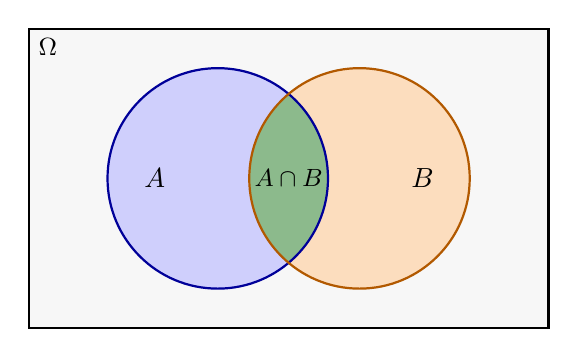
\begin{tikzpicture}
  \draw[thick,fill=gray!6] (-3.3,-1.9) rectangle (3.3,1.9);
  \node[anchor=north west,font=\small] at (-3.3,1.9) {$\Omega$};
  \fill[blue!25,opacity=0.7] (-0.9,0) circle (1.4);
  \fill[orange!35,opacity=0.7] (0.9,0) circle (1.4);
  \begin{scope}
    \clip (-0.9,0) circle (1.4);
    \fill[green!40!black!45] (0.9,0) circle (1.4);
  \end{scope}
  \draw[thick,blue!60!black] (-0.9,0) circle (1.4);
  \draw[thick,orange!70!black] (0.9,0) circle (1.4);
  \node at (-1.7,0) {$A$};
  \node at (1.7,0) {$B$};
  \node[font=\small] at (0,0) {$A\cap B$};
\end{tikzpicture}
\captionof{figure}{Two events $A$ and $B$ inside the sample space $\Omega$. The overlap $A\cap B$ is part of both circles, so it is subtracted once in the addition rule.}\label{fig:pr1_venn}
\end{center}

\begin{example}
During a walking test a robot slips with probability $P(A)=0.10$ and shows a low-battery warning with $P(B)=0.05$. Both happen together with $P(A\cap B)=0.02$. Then
\[
P(A\cup B)=0.10+0.05-0.02=0.13,
\]
so $13\,\%$ of the tests have at least one of the two problems.
\end{example}

\subsection*{Independent events}
Two events are \textbf{independent} if knowing that one happened tells nothing about the other, like two kicks that do not influence each other. In that case
\[
P(A\cap B)=P(A)\cdot P(B).
\]
A \textbf{tree diagram} is a good picture for this. Each branch carries a probability, and the probability of a path is the product along the path. Figure~\ref{fig:pr1_tree} shows two penalties with $P(\text{goal})=0.7$. The four paths together have probability $0.49+0.21+0.21+0.09=1$.

\begin{center}
\begin{tikzpicture}[grow=right,level 1/.style={sibling distance=4.2cm,level distance=3.0cm},level 2/.style={sibling distance=2.0cm,level distance=3.2cm},
  every node/.style={font=\small},edge from parent/.style={draw,-{Stealth},thick}]
  \node[circle,draw,thick,fill=gray!10] {start}
    child { node[draw,rounded corners,fill=red!10] {miss}
      child { node[draw,rounded corners,fill=red!10] {miss}
        edge from parent node[below,font=\scriptsize] {$0.3$} }
      child { node[draw,rounded corners,fill=green!15] {goal}
        edge from parent node[above,font=\scriptsize] {$0.7$} }
      edge from parent node[below left,font=\scriptsize] {$0.3$} }
    child { node[draw,rounded corners,fill=green!15] {goal}
      child { node[draw,rounded corners,fill=red!10] {miss}
        edge from parent node[below,font=\scriptsize] {$0.3$} }
      child { node[draw,rounded corners,fill=green!15] {goal}
        edge from parent node[above,font=\scriptsize] {$0.7$} }
      edge from parent node[above left,font=\scriptsize] {$0.7$} };
  \node[font=\scriptsize,anchor=west] at (7.8,-2.55) {$0.3\cdot0.3=0.09$};
  \node[font=\scriptsize,anchor=west] at (7.8,-0.95) {$0.3\cdot0.7=0.21$};
  \node[font=\scriptsize,anchor=west] at (7.8,0.95)  {$0.7\cdot0.3=0.21$};
  \node[font=\scriptsize,anchor=west] at (7.8,2.55)  {$0.7\cdot0.7=0.49$};
\end{tikzpicture}
\captionof{figure}{Tree diagram of two independent penalties. The probability of a path is the product of the branch probabilities.}\label{fig:pr1_tree}
\end{center}

\begin{example}[Rolling two dice]
Two dice give $6\cdot6=36$ equally likely outcomes, shown in Figure~\ref{fig:pr1_dice}. The sum is $7$ in the six outcomes $(1,6),(2,5),\dots,(6,1)$, so $P(\text{sum}=7)=\frac{6}{36}=\frac16$. Rolling two sixes has probability $\frac16\cdot\frac16=\frac1{36}$.
\end{example}

\begin{center}
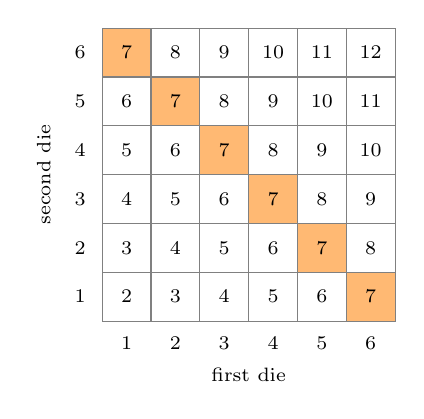
\begin{tikzpicture}[scale=0.62]
  \foreach \da in {1,...,6}{
    \foreach \db in {1,...,6}{
      \pgfmathtruncatemacro{\sm}{\da+\db}
      \ifnum\sm=7
        \fill[orange!55] (\da-1,\db-1) rectangle (\da,\db);
      \fi
      \draw[gray] (\da-1,\db-1) rectangle (\da,\db);
      \node[font=\scriptsize] at (\da-0.5,\db-0.5) {\sm};
    }
  }
  \foreach \da in {1,...,6}{
    \node[font=\scriptsize] at (\da-0.5,-0.45) {\da};
    \node[font=\scriptsize] at (-0.45,\da-0.5) {\da};
  }
  \node[font=\scriptsize] at (3,-1.1) {first die};
  \node[font=\scriptsize,rotate=90] at (-1.2,3) {second die};
\end{tikzpicture}
\captionof{figure}{The $36$ outcomes of two dice. Each field shows the sum. The six orange fields have the sum $7$.}\label{fig:pr1_dice}
\end{center}

\section*{Counting}
For equally likely outcomes we need to \emph{count}. Three tools are enough.

\textbf{Multiplication principle.} If a choice has $a$ possibilities and a second choice has $b$ possibilities, then there are $a\cdot b$ combinations. A robot ID with two letters ($26$ each) followed by three digits ($10$ each) allows $26\cdot26\cdot10\cdot10\cdot10=676\,000$ different IDs.

\textbf{Orderings (permutations).} The number of ways to put $n$ different things in a row is $n!=n\cdot(n-1)\cdots2\cdot1$ (``$n$ factorial''). Three robots can line up in $3!=6$ ways. If we pick only $k$ of $n$ and the order matters, we get $n(n-1)\cdots(n-k+1)$ possibilities. Choosing a captain, a vice-captain and a goalkeeper from $5$ players: $5\cdot4\cdot3=60$.

\textbf{Choosing without order (combinations).} If the order does not matter, the number of ways to choose $k$ of $n$ things is the \textbf{binomial coefficient}
\[
\binom{n}{k}=\frac{n!}{k!\,(n-k)!}.
\]
Choosing $3$ of $5$ players for a drill: $\binom53=\frac{5\cdot4\cdot3}{3\cdot2\cdot1}=10$. Every group of three was counted $3!=6$ times in the $60$ ordered choices, and $60/6=10$. Useful special values: $\binom n0=\binom nn=1$, $\binom n1=n$, and $\binom nk=\binom n{n-k}$.

\begin{example}
A team has $6$ field players. A pair is chosen at random. How likely is it that the pair consists of two specific players $X$ and $Y$? There are $\binom62=15$ pairs, and only one of them is $\{X,Y\}$. So the probability is $\frac1{15}=0.067$.
\end{example}

\begin{aibox}
A probability model is how a robot reasons about an uncertain world: ``the ball is here with probability $0.8$''. Chapter~\ref{ch:cond} shows how a robot updates such numbers when it gets new sensor data, and Chapter~\ref{ch:normal} describes sensor noise with the most important distribution of all.
\end{aibox}

\section*{Practice problems}
\begin{enumerate}[label=\textbf{\thechapter.\arabic*}]
  \item A fair die is rolled. Find (a) $P(\text{odd})$, (b) $P(\text{more than }4)$, (c) $P(\text{not }6)$.
  \item Two fair dice are rolled. Find (a) $P(\text{sum}=7)$, (b) $P(\text{sum}\ge11)$, (c) the probability that both dice show the same number. (Use Figure~\ref{fig:pr1_dice}.)
  \item A robot falls during a walking test with probability $0.08$. What is the probability that it does \emph{not} fall in one test? In three independent tests?
  \item For two events $P(A)=0.6$, $P(B)=0.5$ and $P(A\cap B)=0.3$. Find $P(A\cup B)$ and the probability that neither $A$ nor $B$ happens.
  \item A penalty is scored with probability $0.7$. For three independent kicks find (a) the probability of three goals, (b) the probability of at least one goal, (c) the probability of exactly two goals. (Hint for (c): there are $\binom32=3$ orders in which the two goals can fall.)
  \item A coach picks a captain and a vice-captain from $6$ players. In how many ways can she do it? In how many ways can she choose $2$ of the $6$ players as substitutes?
  \item Compute (a) $5!$, (b) $\binom{6}{2}$, (c) $\binom{10}{3}$, (d) $\binom{8}{8}$.
  \item A die is rolled and a coin is tossed. What is the probability of ``six and heads''?
  \item Write a Python program that estimates $P(\text{sum}=7)$ for two dice with $100\,000$ random rolls. What value do you expect?
  \item[\textbf{\thechapter.10}$\star$] Five people are in a room. Compute the probability that at least two of them have the same birthday (ignore leap years). Hint: use the complement ``all five birthdays are different''.
\end{enumerate}
